\chapter{Aperiodic Servers}
The scheduling algorithms treated in the previous chapter deals with homogeneous sets of tasks, where all computational activities are periodic. Many real-time control applications, however, require both aperiodic and periodic processes, which may also differ for their criticality. Tipically, periodic tasks are time-driven and execute critical control activities with hard timing contraints aimed at guaranteeing regular activation rates. Aperiodic tasks are usually event-driven and may have hard, soft, or non real-time requirements depending on the specific applications.

When dealing with hybrid task sets, the main objective of the kernel is to guarantee the schedulability of all critical tasks in worst-case conditions and provide good average response times for soft and non-real-time activities. Off-line guarantee of event-driven aperiodic tasks with critical timing contraints can be done only by making proper assumptions on the environment; that is, by assuming a maximum arrival rate for each critical event. This implies that aperiodic tasks associated with critical events are characterized by a minimum interarrival time between consecutive instances, which vounds the aperiodic load. Aperiodic tasks characterized by a minimum interarrival time are called sporadic. They are guaranteed under peak-load situations by assuming their maximum arrival rate.

\section{Background Execution}
The simplest method to handle a set of soft aperiodic activities in the presence of periodic tasks is to schedule them in background; that is, when there are not periodic instances ready to execute. The major problem with this technique is that, for high periodic loads, the response time of aperiodic requests can be too long for certain applications. For this reason, background scheduling can be adopted only when the aperiodic activities do not have stringest timing constraints and the periodic load is not high.

The major advantage of background scheduling is its simplicity. In general, only two queues are needed to implement the scheduling mechanism: one (with a higher priority) dedicated to periodic tasks and the other (with a lower priority) reserved for aperiodic requests. The two queueing strategies are independent and can be realized by different algorithms. Tasks are taken from the aperiodic queue only when the periodic queue is empty. The activation of a new periodic instance causes any aperiodic tasks to be immediately preempted.

    \begin{figure}[!h]
        \centering
        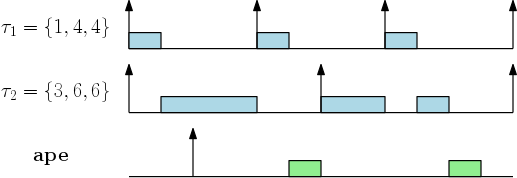
\includegraphics[width = 0.75\textwidth]{images/image02.png}
    \end{figure}

\section{Immediate Execution}
Contrary to the Background Execution, aperiodic tasks are served with the highest priority as soon as they come. This however, might cause deadline misses among the periodic tasks.

\begin{figure}[!h]
    \centering
    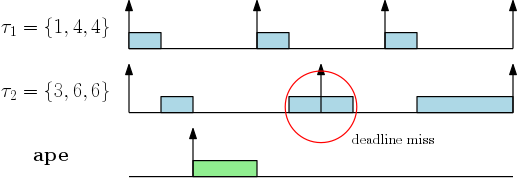
\includegraphics[width = 0.75\textwidth]{images/image03.png}
\end{figure}

Aperiodic Servers are the solution to the problem. Normally we associate two parameters with a server:
\begin{itemize}
    \item $C_s$: capacity
    \item $T_s$: server period
\end{itemize}
Roughly speaking, the idea is that the served tasks receive no more that $C_s$ time units every $T_s$. How this is done depends on the specific server technology.


The server is scehduled as any periodic tasks. Priorities are manipulated in favour of the server. Tasks inside the server can be queued with an arbitrary discipline.
\section{Polling Servers (PS)}
The average response time of aperiodic tasks can be improved with respect to background scheduling through the use of a \side{server}, that is, a periodic task whose purpose is to service aperiodic requests as soon as possible. Like any periodic task, a server is characterized by a \side{server period} $T_s$ and a computation time $C_s$, called \side{server capacity}, or \side{server budget}. In general, the server is scheduled with the same algorithm used for the periodic tasks, and once active, it serves the aperiodic requests within the limit of its budget. The ordering of aperiodic requests does not depend on the scheduling algorithm used for periodic tasks, and it can be done by arrival time, computation time, deadline or any other parameter.


\begin{figure}[!h]
    \centering
    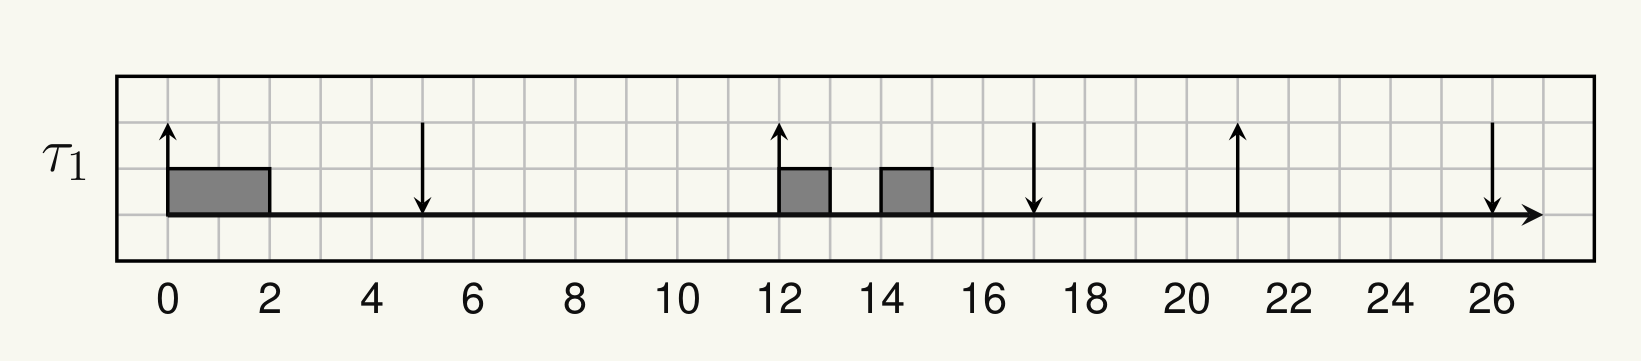
\includegraphics[width = 0.75\textwidth]{images/image04.png}
\end{figure}


The \side{Polling Server (PS)} is an algorithm based on such an approach. At regular intervals equal to the period $T_s$, PS become active and serves the pending aperiodic requests withing the limit of its capacity $C_s$. If no aperiodic requests are pending, PS suspends itself until the beginning of its next period, and the budget originally allocated for aperiodic service is discharged and given periodi tasks.\\
Note that if an aperiodic request arrives just after the server has suspended, it must wait until beginning of the next period, when the server capacity is replenished at its full value.

\section{Deferrable Servers (DS)}
The \side{Deferrable Server (DS)} algorithm is a service technique introduced by Lehoczky, Sha, and Strosnider to improve the average response time of aperiodic requests with respect to polling service. As the Polling Server, the DS algorithm creates a periodic task (usually having a high priority) for servicing aperiodic requests. However, unlike polling, DS preserves its capacity if no requests are pending upon the invocation of the server. The capacity is maintained until the end of the period, so that aperiodic requests can be services at the same server's priority at anytime, as long as the capacity has not been exhausted. At the beginning of any server period the capacity is replenished at its full value.


\begin{figure}[!h]
    \centering
    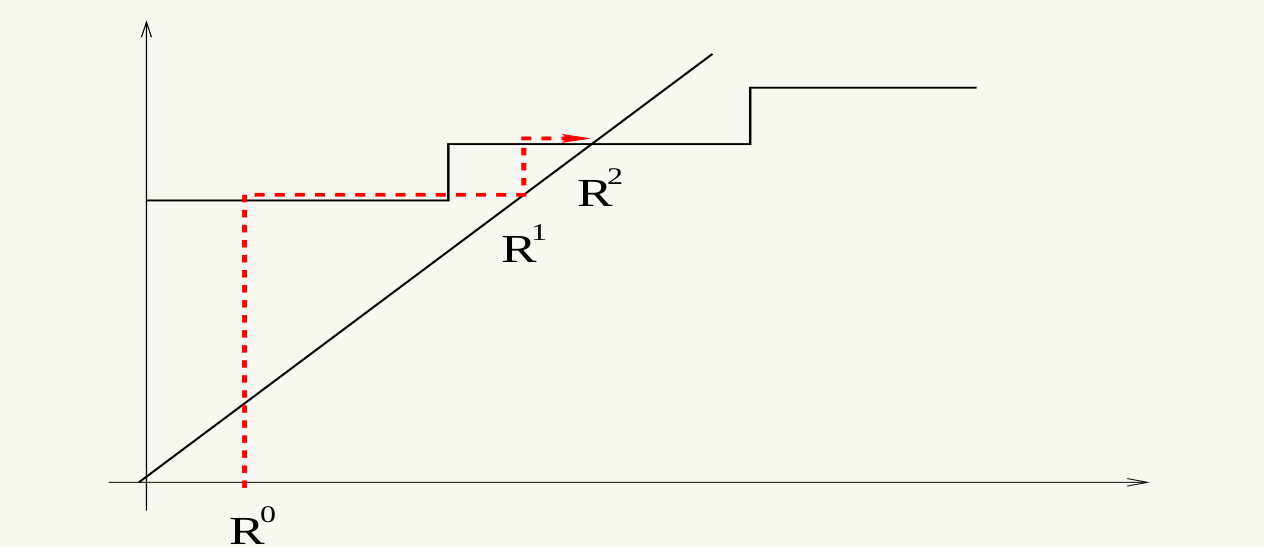
\includegraphics[width = 0.75\textwidth]{images/image05.png}
\end{figure}


DS provides much better aperiodic responsiveness than polling, since it preserves the capacity until is needed. Shorter response times can be achieved by creating a Deferrable Server having the highest priority among the periodic tasks.

\section{Sporadic Servers (SS)}

The \side{Sporadic Server (SS)} algorithm is another technique which allow the enhancement of the average response time of aperiodic  tasks without degrading the utilization bound of the periodic task set.

The SS algorithm creates a high-priority task for servicing aperiodic requests and, like DS, preserves the server capacity at its high-priority level until an aperiodic request occurs. However, SS differs from DS in the way it replenishes its capacity. Whereas DS periodically replenish their capacity to full value at the beginning of each server period, SS replenishes its capacity only after it has been consumed by aperiodic task execution.

In order to simplify the description of the replenishment method used by SS, the following terms are defined:
\begin{itemize}
    \item{\makebox[1.5cm]{$P_{exe}$\hfill} It denotes the priority level of the task that is currently executing}
    \item{\makebox[1.5cm]{$P_{s}$\hfill} It denotes the priority level associated with SS}
    \item{\makebox[1.5cm]{\textbf{Active}\hfill}SS is said to be active when $P_{exe}\ge P_s$}
    \item{\makebox[1.5cm]{\textbf{Idle}\hfill}SS is said to be idle when $P_{exe} < P_s$}
    \item{\makebox[1.5cm]{\textbf{RT}\hfill} It denotes the replenishment time at which the SS capacity will be replenished}
    \item{\makebox[1.5cm]{\textbf{RA}\hfill}It denotes the replenishment amount that will be added to the capacity at time RT}
\end{itemize}

Using this terminology, the capacity $C_s$ consumed by aperiodic requests is replenished according to the following rules:
\begin{itemize}
    \item The replenishment time RT is set as soon as SS becomes active and $C_s > 0$. Let $t_a$ be such a time. The value of RT is set equal to $T_a$ plus the server period
     \[RT = t_a + T_s\]
    \item The replenishment amount RA to be done at time RT is computed when SS becomes idle or $C_s$ has been exhausted. Let $t_I$ be such ta time. The value of RA is set equal to the capacity consumed withing the interval $[t_a, t_I]$ 
\end{itemize}

\section{Constant Bandwidth Servers (CBS)}
In this section we present a novel service mechanism, called \side{Constant Bandwidth Server (CBS)}, which efficiently implements a bandwidth reservation strategy. The Constant Bandwidth Server guarantees that, if $U_s$ is the fraction of processor time assigned to a server (i.e. its bandwidth), its contribution to the total utilization factor is no greater thatn $U_s$, even in the presence of overloads. 

The basic idea behind the CBS mechanism can be explained as follows: when a new job enters the system, it is assigned a suitable scheduling deadline (to keep its demand within the reserved bandwidth) and it is inserted in the EDF ready queue. If the job tries to execute more than expected, its deadline is postponed (i.e. its priority is decreased) to reduce the interference on the other tasks. Note that by postponing the deadline, the task remains eligible for execution. In this way, the CBS behaves as a work conserving algorithm, exploiting the available slack in an efficient (deadline-based) way, thus prividing better responsiveness with respect to non-work conserving algorithms and to other reservation approaches that schedule the extra portions of jobs in background.

If a subset of tasks is handled by a single server, all the tasks in that subset will share the same bandwidth, so there is no isolation among them. Novertheless, all the other tasks in the system are protected agains overruns occurring in the subset.

In order not to miss any hard deadline, the deadline assignment rules adopted by the server must be carefully designed.

\definition{Constant Bandwidth Server}{
    A CBS is characterized by three main quantities:
    \begin{itemize}
        \item an ordered pair $(Q_s, T_s)$ assigned by the user.\\
        Where $Q_s$ is the maximum budget and $T_s$ is the period of the server. The ratio
        \[U_s = \cfrac{Q_s}{T_s}\]
        is denotes as the server bandwidth.
        \item The current budget $q_s$ (initialized to 0) managed by the server.
        \item The scheduling deadline $d_s$ (initialized to 0) managed by the server.
    \end{itemize}
    Each served job $J_k$ is assigned a dynamic deadline equal to the current server deadline.\\
    Whenever a served job executes, the server budget $q_s$ is decreased by the same amount.
}

The CBS acts considering the following procedures:
\begin{enumerate}
    \item When the server budget is exhausted (i.e. $q_s = 0$), the server budget is recharged at the maximum value $Q_s$ and a new server deadline is generated as $d_s = d_s + T_s$. Note that there are no finite intervals of time in which the budget is equal to zero.
    \item When a job $J_k$ arrives and the server is active the request is enqueued in a queue of pending jobs according to a given (arbitrary) discipline.
    \item When a job $J_k$ arrives and the server is idle, if $q_s \ge (d_s - r_k) U_s$ the server generates a new deadline $d_s = r_k + T_s$ and $q_s$ is recharged at the maximum value $Q_s$, otherwise the job is served with the last server deadline $d_s$ using the current budget.
    \item When a job finishes, the next pending job, if any, is served using the current budget and deadline. If there are no pending jobs, the server becomes idle.
\end{enumerate}

Hence, the server behaviour can be described by the algorithm:
\begin{algorithm}
    \begin{algorithmic}
        \STATE At arrival of job $J_k$ at time $r_k\,\rightarrow$ Assign $d_s$ 
        \IF{$\exists$ pending aperiodic request}
        \STATE enqueue $J_k$
        \ELSE
        \IF{($q_s \ge (d_s - r_k)\,U_s$)}  % not enough budget left
        \STATE $q_s \leftarrow Q_s$       % replanish the budget
        \STATE $d_s \leftarrow r_k + T_s$ % generate new deadline
        \ELSE
        \STATE Continue to use the budget $q_s$ with deadline $d_s$
        \ENDIF
        \ENDIF
    \end{algorithmic}
\end{algorithm}


\subsection{CBS Properties}
The proposed CBS service mechanism presents some interesting properties that make it suitable for supporting applications with highly variable computation times. The most important one, the \side{temporal isolation property}, is formally expressed as follows:

\theorem{}{The CPU utilization of a CBS with parameters $(Q_s, T_s)$ is 
\[U_s = \cfrac{Q_s}{T_s}\]
 independently from the computation times and the arrival pattern of the served jobs.}

 \lemma{}{Given a set of $n$ periodic hard tasks with processor utilization $U_p$ and a set of $m$ CBSs with processor utilization 
 \[U_s = \sum_{i=1}^m U_{si}\]
 the whole set is schedulable by EDF if and only if
 \[U_p + U_s \le 1\]
 }

 The temporal isolation property allows us to use a bandwidth reservation strategy to allocate a fraction of the CPU time to soft tasks whose computation time cannot be easily bounded. The most imporant consequence of this result is that soft tasks can be scheduled together with hard tasks without affecting the a priori guarantee, even in the case in which the execution time of the soft tasks are not known or the soft requests exceed the expected load.\\
 Another general technique used in real-time systems for limiting the effects of overruns in tasks with variable computation times is the \side{resource reservation paradigm}. According to this method, each task is assigned a fraction of the processor bandwidth, just enough to satisfy its timing containts. The kernel, however, must prevent each task from consuming more that the requested amount to protect the other tasks in the systems (\side{temporal protection}). In this way, a task receiving a fraction $U_i$ of the total processor bandwidth behaves as it were executing alone on a slower processor with a speed equal to $U_i$ times the full speed. The advantage of this method is that each task can be guaranteed in isolation, independently of the behavior of the other tasks.

 A simple and effective mechanism for implementing resource reservation in a real-time system is to reserve each task $\tau_i$ a specified amount of CPU time $Q_i$ in every reservation period $T_s$.


